\documentclass{article}
\usepackage[utf8]{inputenc}
\usepackage{authblk}
\usepackage{graphicx} % Lib de importar e tratar imagem
\usepackage[english,brazil]{babel} % Manter dois idiomas
\usepackage{fancyhdr} % Configuração das paginas
\usepackage{float}
\usepackage{xcolor}
\usepackage{titlesec}
\usepackage{background} % Componente de Watermark
\usepackage{hyperref}
\usepackage{verbatim}
\usepackage[a4paper, left=2cm, right=2cm]{geometry}
\usepackage[most]{tcolorbox}
\usepackage{upquote}

\newcommand{\shellcmd}[1]{\\\indent\indent\texttt{\footnotesize\# #1}\\}

% Definir as características do hyperlink
\hypersetup{
    colorlinks=true,
    linkcolor=blue,
    filecolor=magenta,      
    urlcolor=cyan,
    pdftitle={Overleaf Example},
    pdfpagemode=FullScreen,
}

%Função para diminuir tamanho da fonte
\newcommand{\changefont}{%
    \fontsize{9}{12}\selectfont
}

%Document Layout Config
\pagestyle{fancy}
\setlength\headheight{26pt}
\setlength\parindent{0pt}
\fancyhf{}

% Header Config
\fancyhead[RO]{Conceitos de Criptografia}
\fancyhead[LO]{\includegraphics[width=0.7cm]{Logo.png}}

% Footer Config
\renewcommand{\footrulewidth}{0.4pt} % Inserir linha no final da pagina "pre-footer"
\fancyfoot[RO]{\includegraphics[width=0.7cm]{Logo.png}}

%Document Specification
\title{Conceitos de Criptografia}
\author{senhasegura}
\affil{Departamento de Segurança e Inovação - SEGi9}
\date{}
\graphicspath{ {img/} }

%Capa
\begin{document}
\NoBgThispage % Ignorar background na capa
\maketitle
\begin{center}

\includegraphics{logo.png}
\end{center}
\begin{center}
\textbf{\LARGE \\PÚBLICO}
\end{center}
\pagenumbering{gobble} % Não contar como página a capa
\pagebreak

% Background a partir da segunda pagina
\backgroundsetup{contents=
\includegraphics{logo.png}, scale=1.5, opacity=0.15, angle=0} % marca d'agua

%Resumo Executivo
\section*{\centering{Resumo Executivo}}
\vspace*{\fill}
\large{Este texto tem como objetivo descrever os principais conceitos da área de segurança, com foco especial na área de criptografia.}
\vspace*{\fill}
\fancyfoot[CO]{senhasegura\\ \changefont Qualquer reprodução ou distribuição é estritamente proibida sem a aprovação prévia por escrito da empresa MT4.}
\pagebreak

%Sumario
\tableofcontents
\pagebreak

%Texto
\fancyfoot[CO]{\thepage\\\changefont Qualquer reprodução ou distribuição é estritamente proibida sem a aprovação prévia por escrito da empresa MT4.}
\pagenumbering{arabic}

% Página
\section{Princípios}
A segurança da informação é um campo fundamental no mundo digital atual, onde a proteção dos dados e informações é essencial para a manutenção da privacidade e a confiabilidade das operações.\\
Dentro deste contexto, existem quatro pilares importantes que sustentam a segurança da informação: Conhecimento Zero, Confidencialidade, Integridade e Autenticidade. Esses pilares são fundamentais para garantir a proteção adequada dos dados e a confiança nas transações e comunicações. A seguir, vamos explorar cada um desses conceitos:

\begin{itemize}
	\item Conhecimento Zero
	\item Confidencialidade
	\item Integridade
	\item Autenticidade
\end{itemize}

\pagebreak

% Página
\section{Conhecimento Zero}

O conceito de Conhecimento Zero, ou Zero Knowledge, refere-se a um modelo de segurança onde o provedor de serviços não possui acesso às informações confidenciais armazenadas pelos usuários. Todas as credenciais, como senhas, notas seguras e outros dados sensíveis, são criptografadas localmente no dispositivo do usuário antes de serem enviadas e armazenadas nos servidores.

\subsection{Funcionamento do Conhecimento Zero}

\begin{enumerate}
	\item Criação e Armazenamento de Credenciais
		\begin{itemize}
			\item O usuário cria suas credenciais (senhas, notas seguras, etc.) no aplicativo.
			\item Antes de qualquer dado ser transmitido para os servidores, ele é criptografado localmente utilizando uma chave derivada da Senha Mestra do usuário.
		\end{itemize}
	\item Criptografia Local
		\begin{itemize}
			\item A Senha Mestra é utilizada para gerar uma chave criptográfica.
			\item Esta chave criptográfica é então utilizada para criptografar todos os dados do usuário localmente no dispositivo.
			\item Os dados criptografados são enviados para os servidores para armazenamento seguro.
		\end{itemize}
	\item Armazenamento Seguro
		\begin{itemize}
			\item Nos servidores, apenas os dados criptografados são armazenados.
			\item O servidor não possui acesso à Senha Mestra do usuário, nem à chave derivada da mesma. Isso significa que, mesmo que os servidores sejam comprometidos, os dados dos usuários permanecem inacessíveis e seguros.
		\end{itemize}
	\item Descriptografia Local
		\begin{itemize}
			\item Quando o usuário precisa acessar suas credenciais, os dados criptografados são baixados do servidor e descriptografados localmente no dispositivo, utilizando novamente a Senha Mestra.
			\item Este processo garante que apenas o usuário, que possui conhecimento da Senha Mestra, pode acessar suas informações confidenciais.
		\end{itemize}
\end{enumerate}

\pagebreak

% Página
\section{Confidencialidade}

A Confidencialidade refere-se à garantia de que as informações são acessíveis apenas por pessoas autorizadas. Em outras palavras, é a proteção contra a divulgação não autorizada de dados. Este pilar é essencial para manter a privacidade dos dados pessoais e sensíveis, como informações financeiras, médicas ou estratégicas de uma organização. Técnicas de criptografia são amplamente utilizadas para garantir a confidencialidade, assegurando que, mesmo que os dados sejam interceptados, eles não possam ser lidos ou compreendidos por indivíduos não autorizados.

\subsection{Algoritmo Simétrico}

Entre os diversos tipos de algoritmos de criptografia, o algoritmo de criptografia simétrica é um dos mais comuns e amplamente utilizados. Neste tipo de algoritmo, a mesma chave(K) é utilizada tanto para criptografar(C), gerando a mensagem cifrada(M), quanto para descriptografar(D) os dados, gerando o Texto Plano(T).\\

A Figura \ref{fig:algoritmo_simetrico} ilustra o funcionamento do algoritmo de criptografia simétrica. Para mostrar o funcionamento do algoritmo, vamos considerar três personagens: \textbf{Alice}, \textbf{Bob} e \textbf{Eva}. Alice e Bob desejam se comunicar de forma segura, enquanto Eva deseja ler a mensagem trocadas entre eles.

\begin{figure}[H]
	\centering
	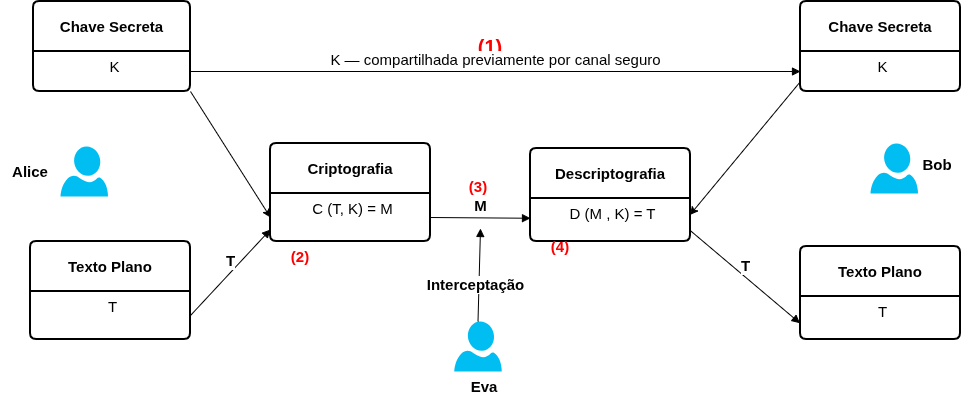
\includegraphics[scale=0.45]{algoritmo_simetrico.png}
	\caption{Funcionamento do algoritmo de criptografia simétrico}
	\label{fig:algoritmo_simetrico}
\end{figure}

\pagebreak
\textbf{Funcionamento do Algoritmo de Criptografia Simétrico}

\begin{enumerate}
	\item Alice e Bob precisam obter a mesma chave secreta (K) por um mecanismo seguro antes de trocar mensagens. O comando abaixo gera uma chave aleatória de 256 bits para o exemplo; executá-lo em Alice não entrega automaticamente uma cópia a Bob.
	\begin{tcolorbox}[width=\textwidth]
		{\normalsize
			\begin{verbatim}
			$ umask 077
			$ openssl rand -hex 32 > K.hex
			\end{verbatim}
		}
	\end{tcolorbox}
	\item Quando Alice deseja enviar o Texto Plano(T) para Bob, ela utiliza AES-256-CBC, a Chave Secreta(K) e um IV aleatório para gerar o Texto Cifrado(M). O IV não é secreto e deve acompanhar o texto cifrado; gere um IV novo e imprevisível para cada cifragem. Este exemplo demonstra apenas confidencialidade: em produção, prefira uma cifra autenticada (AEAD), como AES-GCM, ou combine CBC com um MAC usando uma chave independente e autentique o IV e o texto cifrado antes de decifrar.
	\begin{tcolorbox}[width=\textwidth]
		{\normalsize
			\begin{verbatim}
			$ IV_HEX=$(openssl rand -hex 16)
			$ printf '%s' "$IV_HEX" > M.iv
			$ openssl enc -aes-256-cbc -K "$(cat K.hex)" -iv "$IV_HEX" \
			  -in T.txt -out M.enc
			\end{verbatim}
		}
	\end{tcolorbox}
	\item Alice envia o Texto Cifrado(M) e o IV para Bob através de um canal de comunicação inseguro. Se Eva apenas interceptar esses dados e a chave permanecer secreta, ela não deverá conseguir recuperar a mensagem original. Como CBC sozinho não autentica os dados, um atacante ativo ainda pode alterar o texto cifrado ou o IV sem que a alteração seja detectada de forma confiável.
	\item Ao receber o Texto Cifrado(M), Bob utiliza o mesmo algoritmo de Descriptografia(D) e a Chave Secreta(K) para transformar o Texto Cifrado(M) de volta ao Texto Plano(T).
	\begin{tcolorbox}[width=\textwidth]
		{\normalsize
			\begin{verbatim}
			$ openssl enc -d -aes-256-cbc -K "$(cat K.hex)" -iv "$(cat M.iv)" \
			  -in M.enc -out T.txt
			\end{verbatim}
		}
	\end{tcolorbox}
\end{enumerate}

A principal vantagem dos algoritmos de criptografia simétrica é sua eficiência e velocidade, especialmente em comparação com os algoritmos de criptografia assimétrica. No entanto, Alice e Bob precisam estabelecer a chave secreta com segurança. Se Eva descobrir essa chave, poderá decifrar as mensagens protegidas por ela.\\

Esses comandos são didáticos: o arquivo K.hex contém a chave em claro, e a opção \texttt{-K} passa a chave como argumento do processo, onde ela pode ficar visível durante a execução. Em produção, use uma biblioteca criptográfica e um mecanismo de armazenamento e uso de chaves que evitem essa exposição. Alice e Bob podem provisionar a chave por um canal protegido ou estabelecê-la por um protocolo autenticado de acordo de chaves.\\

\subsection{Algoritmo Assimétrico}

O algoritmo de criptografia assimétrica é uma técnica fundamental no campo da segurança e criptografia. Diferente dos algoritmos de criptografia simétrica, que utilizam a mesma chave para criptografar e descriptografar os dados, os algoritmos assimétricos usam um par de chaves: uma chave pública(KPu) e uma chave privada(KPr). Vamos explorar o funcionamento desse algoritmo através dos personagens Alice, Bob e Eva exemplificado pela Figura \ref{fig:algoritmo_assimetrico}.

\begin{figure}[H]
	\centering
	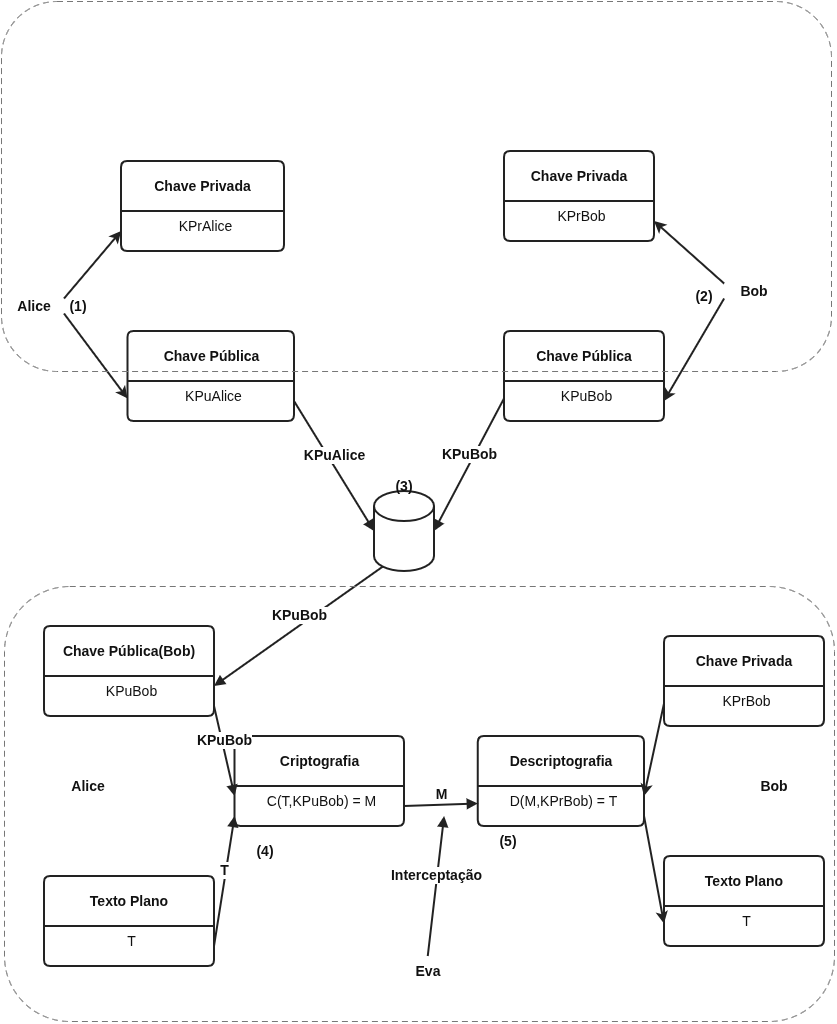
\includegraphics[scale=0.45]{algoritmo_assimetrico.png}
	\caption{Funcionamento do algoritmo de criptografia assimétrico}
	\label{fig:algoritmo_assimetrico}
\end{figure}

\pagebreak

\textbf{Funcionamento do Algoritmo de Criptografia Assimétrico}

\begin{enumerate}
	\item Alice gera um par de chaves, Chave Pública(KPuAlice) e Chave Privada(KPrAlice);
	\begin{tcolorbox}[width=\textwidth]
		{\normalsize
			\begin{verbatim}
			$ openssl genpkey -algorithm RSA -out KPrAlice.pem -pkeyopt rsa_keygen_bits:2048
			$ openssl rsa -pubout -in KPrAlice.pem -out KPuAlice.pem
			\end{verbatim}
		}
	\end{tcolorbox}
	\item Bob gera um par de chaves, Chave Pública(KPuBob) e Chave Privada(KPrBob);
	\begin{tcolorbox}[width=\textwidth]
		{\normalsize
			\begin{verbatim}
			$ openssl genpkey -algorithm RSA -out KPrBob.pem -pkeyopt rsa_keygen_bits:2048
			$ openssl rsa -pubout -in KPrBob.pem -out KPuBob.pem
			\end{verbatim}
		}
	\end{tcolorbox}
	\item Tanto Alice quanto Bob enviam as suas respectivas chaves públicas, KPuAlice e KPuBob, para um servidor de chave pública;
	\item Antes de usar a chave pública recuperada do servidor, Alice deve verificar por um meio confiável que ela realmente pertence a Bob, por exemplo, validando um certificado digital ou comparando sua impressão digital por um canal autenticado. A presença da chave no servidor, por si só, não comprova essa associação: um atacante que substitua a chave de Bob pela sua própria pode interceptar a comunicação;
	\item Quando Alice deseja enviar um Texto Plano (T) curto para Bob, ela utiliza a Chave Pública do Bob (KPuBob.pem) para gerar o Texto Cifrado (M). Com RSA de 2048 bits e OAEP/SHA-256, a entrada deve ter no máximo 190 bytes. Para mensagens maiores, usa-se criptografia híbrida: Alice cifra a mensagem com uma chave simétrica aleatória usando uma cifra autenticada, como AES-GCM, e cifra essa chave simétrica com a chave pública de Bob.
	\begin{tcolorbox}[width=\textwidth]
		{\normalsize
			\begin{verbatim}
			$ openssl pkeyutl -encrypt -inkey KPuBob.pem -pubin -in T.txt -out M.bin \
			  -pkeyopt rsa_padding_mode:oaep -pkeyopt rsa_oaep_md:sha256
			\end{verbatim}
		}
	\end{tcolorbox}
	\item Ao receber o Texto Cifrado(M), o Bob utiliza sua Chave Privada(KPrBob) para descriptografá-la obtendo o Texto Plano(T).
	\begin{tcolorbox}[width=\textwidth]
		{\normalsize
			\begin{verbatim}
			$ openssl pkeyutl -decrypt -inkey KPrBob.pem -in M.bin -out T.txt \
			  -pkeyopt rsa_padding_mode:oaep -pkeyopt rsa_oaep_md:sha256
			\end{verbatim}
		}
	\end{tcolorbox}
\end{enumerate}

Se Alice usar uma chave pública de Bob cuja associação com ele foi verificada, e Bob proteger sua chave privada, a cifragem com RSA-OAEP protege a confidencialidade contra Eva, mesmo que ela intercepte o texto cifrado. Esse fluxo, por si só, não comprova que a mensagem foi enviada por Alice: qualquer pessoa que conheça a chave pública de Bob pode cifrar mensagens para ele. Para autenticar a origem, Alice deve assinar a mensagem com sua chave privada, e Bob deve verificar a assinatura usando uma chave pública de Alice cuja associação também seja confiável.\\

Na criptografia híbrida, a cifra autenticada permite detectar alterações no conteúdo cifrado, mas não identifica quem o produziu. A assinatura digital fornece essa verificação de origem, desde que a chave pública do remetente esteja autenticada.

\subsection{Key-Encryption-Key (KEK)}

O conceito de Key-Encryption-Key(KEK), ou Chave de Criptografia de Chaves, é uma tecnologia utilizada para proteger outras chaves criptográficas, como por exemplo, o uso da KEK para proteger as Chaves de Criptografia de Dados(DEK). Ao usar uma KEK para resguardar as DEKs, adiciona-se uma camada extra de segurança ao sistema, melhorando significativamente sua proteção como um todo.\\

A Figura \ref{fig:kek} ilustra o funcionamento e da utilização do conceito KEK.

\begin{figure}[H]
	\centering
	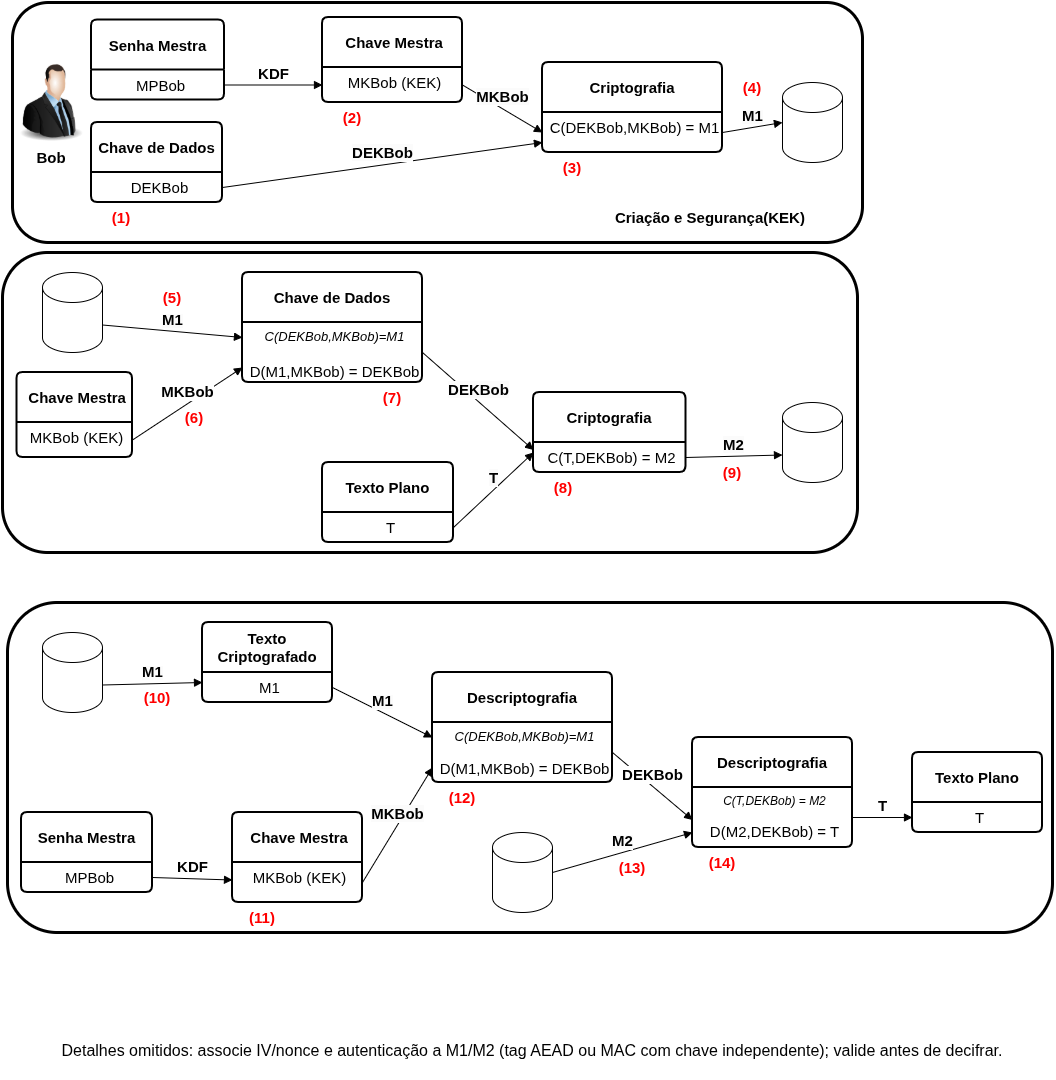
\includegraphics[scale=0.45]{kek.png}
	\caption{Funcionamento do conceito Key-Encryption-Key (KEK)}
	\label{fig:kek}
\end{figure}

\textbf{- Criptografar a Chave de Dados(DEKBob)}

\begin{enumerate}
	\item Bob cria a Chave de Dados (DEKBob.bin);
	\begin{tcolorbox}[width=\textwidth]
		{\normalsize
			\begin{verbatim}
			$ openssl rand -out DEKBob.bin 32
			\end{verbatim}
		}
	\end{tcolorbox}
	\item Bob deriva a Chave Mestra (MKBob.hex) a partir da Senha Mestra (MPBob), usando PBKDF2, SHA-256, 600.000 iterações e um salt aleatório de 128 bits;
	\begin{tcolorbox}[width=\textwidth]
		{\footnotesize
			\begin{verbatim}
			$ read -rs MASTER_PASSWORD
			$ SALT_HEX=$(openssl rand -hex 16)
			$ printf '%s' "$SALT_HEX" > MKBob.salt
			$ openssl kdf -keylen 32 -kdfopt digest:SHA256 \
			  -kdfopt pass:"$MASTER_PASSWORD" -kdfopt salt:"$SALT_HEX" \
			  -kdfopt iter:600000 PBKDF2 | tr -d ':\n' > MKBob.hex
			\end{verbatim}
		}
	\end{tcolorbox}
	\item Aplicando o conceito de KEK, a Chave de Dados (DEKBob.bin) é criptografada com a Chave Mestra do Bob (MKBob.hex), gerando o Texto Cifrado M1. O IV acompanha o texto cifrado;
	\begin{tcolorbox}[width=\textwidth]
		{\scriptsize
			\begin{verbatim}
			$ IV_HEX=$(openssl rand -hex 16)
			$ printf '%s' "$IV_HEX" > M1.iv
			$ openssl enc -aes-256-cbc -K "$(cat MKBob.hex)" -iv "$IV_HEX" \
			  -in DEKBob.bin -out M1.enc
			\end{verbatim}
		}
	\end{tcolorbox}
	\item Bob envia o Texto Cifrado M1 para o servidor;
\end{enumerate}

\textbf{- Criptografar o Texto Plano(T) com uma Chave de Dados DEKBob}

\begin{enumerate}
	\setcounter{enumi}{4} % Define o contador para começar do número 5
	\item Bob recupera o Texto Cifrado M1 do servidor;
	\item Bob possui sua Chave Mestra (MKBob.hex);
	\item Bob descriptografa o Texto Cifrado M1 para obter acesso à sua Chave de Dados (DEKBob.bin);
	\begin{tcolorbox}[width=\textwidth]
		{\scriptsize
			\begin{verbatim}
			$ openssl enc -d -aes-256-cbc -K "$(cat MKBob.hex)" -iv "$(cat M1.iv)" \
			  -in M1.enc -out DEKBob.bin
			\end{verbatim}
		}
	\end{tcolorbox}
	\item Bob utiliza sua Chave de Dados (DEKBob.bin) e um IV aleatório para cifrar o Texto Plano (T), gerando o Texto Cifrado M2;
	\begin{tcolorbox}[width=\textwidth]
		{\small
			\begin{verbatim}
			$ DEK_HEX=$(od -An -v -tx1 DEKBob.bin | tr -d ' \n')
			$ IV_HEX=$(openssl rand -hex 16)
			$ printf '%s' "$IV_HEX" > M2.iv
			$ openssl enc -aes-256-cbc -K "$DEK_HEX" -iv "$IV_HEX" \
			  -in T.txt -out M2.enc
			\end{verbatim}
		}
	\end{tcolorbox}
	\item Bob envia o Texto Cifrado M2 para o servidor;
\end{enumerate}

\textbf{- Descriptografar o Texto Cifrado M2 para obter o Texto Plano(T)}

\begin{enumerate}
	\setcounter{enumi}{9} % Define o contador para começar do número 10
	\item Bob recupera o Texto Cifrado M1 do servidor;
	\item Bob possui sua Chave Mestra (MKBob.hex);
	\item Bob descriptografa o Texto Cifrado M1 com sua Chave Mestra (MKBob.hex) para obter acesso à sua Chave de Dados (DEKBob.bin);
	\begin{tcolorbox}[width=\textwidth]
		{\scriptsize
			\begin{verbatim}
			$ openssl enc -d -aes-256-cbc -K "$(cat MKBob.hex)" -iv "$(cat M1.iv)" \
			  -in M1.enc -out DEKBob.bin
			\end{verbatim}
		}
	\end{tcolorbox}
	\item Bob recupera o Texto Cifrado M2 do servidor;
	\item Bob descriptografa o Texto Cifrado M2 com sua Chave de Dados (DEKBob.bin) para obter acesso ao Texto Plano (T);
	\begin{tcolorbox}[width=\textwidth]
		{\small
			\begin{verbatim}
			$ DEK_HEX=$(od -An -v -tx1 DEKBob.bin | tr -d ' \n')
			$ openssl enc -d -aes-256-cbc -K "$DEK_HEX" -iv "$(cat M2.iv)" \
			  -in M2.enc -out T.txt
			\end{verbatim}
		}
	\end{tcolorbox}
\end{enumerate}

O Key-Encryption-Key (KEK) é um componente essencial em arquiteturas de segurança que exigem a proteção de múltiplas chaves criptográficas \textbf{DEK}. Seu uso permite a proteção eficiente das DEKs, garantindo a segurança dos dados criptografados e simplificando a gestão das chaves. Implementar KEKs corretamente é necessário para manter a integridade e a confidencialidade dos dados em qualquer sistema seguro.\\

\subsection{Key Derivation Functions (KDF)}

As funções de derivação de chaves (Key Derivation Functions - KDF) são um componente essencial na segurança e criptografia de dados. Estas funções são utilizadas para transformar um segredo inicial, como uma senha ou uma chave de criptografia, em uma ou mais chaves criptográficas que podem ser usadas para cifrar dados ou autenticar mensagens.\\

O processo de derivação de chave geralmente envolve a aplicação de uma função matemática que transforma a entrada original em uma chave na saída. A Figura \ref{fig:kdf} exemplifica o processo de derivação da Senha Mestra em uma Chave Mestra. Esta transformação é feita para garantir que a chave resultante seja segura e apropriada para uso em operações criptográficas. Os KDFs são projetados para serem resistentes a ataques, como ataques de força bruta, onde um atacante tenta todas as combinações possíveis até encontrar a correta.

\begin{figure}[H]
	\centering
	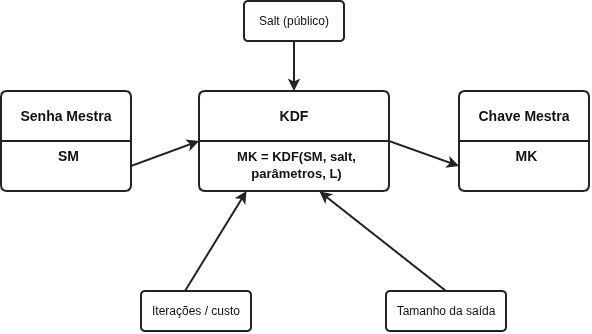
\includegraphics[scale=0.45]{kdf.png}
	\caption{Funcionamento do conceito Key Derivation Functions (KDF)}
	\label{fig:kdf}
\end{figure}

Um exemplo comum de KDF é a função PBKDF2 (Password-Based Key Derivation Function 2), definida no padrão PKCS \#5. O PBKDF2 usa um algoritmo de hash criptográfico, como SHA-256, e um determinado número de iterações para transformar a senha inicial em uma chave derivada. O processo de iteração aumenta a dificuldade de ataques de força bruta, pois cada tentativa de senha requer várias operações de hash.\\

Além de PBKDF2, há também Argon2, uma KDF moderna que ganhou o Password Hashing Competition (PHC) em 2015. Argon2 é altamente configurável, permitindo ajustes precisos em termos de memória, tempo de processamento e paralelismo, oferecendo um equilíbrio entre segurança e performance.\\

O uso de KDFs é essencial em sistemas onde a segurança da chave criptográfica é crucial. Sem um KDF adequado, as chaves derivadas podem ser vulneráveis a diversos tipos de ataques, comprometendo a integridade e confidencialidade dos dados. Portanto, a escolha e implementação corretas de uma KDF robusta são fundamentais para a segurança criptográfica eficaz.\\

Abaixo estão exemplos de comandos que utilizam o OpenSSL para realizar o processo de Key Derivation Functions (KDF), que é usado para derivar uma chave criptográfica a partir de uma senha ou outra informação inicial.

\begin{enumerate}
	\item Derivar uma chave de 256 bits usando PBKDF2 e salvar sua representação hexadecimal localmente. O salt é armazenado junto dos metadados necessários à derivação.
	\begin{tcolorbox}[width=\textwidth]
	{\footnotesize
		\begin{verbatim}
			$ read -rs MASTER_PASSWORD
			$ SALT_HEX=$(openssl rand -hex 16)
			$ printf '%s' "$SALT_HEX" > MKBob.salt
			$ openssl kdf -keylen 32 -kdfopt digest:SHA256 \
			  -kdfopt pass:"$MASTER_PASSWORD" -kdfopt salt:"$SALT_HEX" \
			  -kdfopt iter:600000 PBKDF2 | tr -d ':\n' > MKBob.hex
		\end{verbatim}
	}
	\end{tcolorbox}
\end{enumerate}

\pagebreak

% Página
\section{Integridade}

A Integridade diz respeito à precisão e consistência das informações ao longo de seu ciclo de vida. Este pilar assegura que os dados não sejam alterados de forma indevida, seja por erros acidentais ou por ações maliciosas. A integridade é mantida através de mecanismos de verificação, como somas de verificação, assinaturas digitais e funções de hash. Esses métodos permitem que qualquer alteração nos dados seja detectada, garantindo que a informação recebida é exatamente a mesma que foi enviada originalmente, sem modificações não autorizadas.
\subsection{Hash}

Um hash é uma função que transforma uma entrada de dados (que pode variar de alguns bytes a grandes volumes de dados) em uma saída de tamanho fixo, geralmente representada como uma sequência de caracteres alfanuméricos. Esta transformação é determinística, o que significa que a mesma entrada sempre produzirá a mesma saída.\\

Alguns exemplos de algoritmos hash populares incluem a família de algoritmos SHA-2 (Secure Hash Algorithm 2), que inclui SHA-224, SHA-256, SHA-384 e SHA-512. Os algoritmos SHA-2 produzem hashes de diferentes tamanhos, sendo o SHA-256 e o SHA-512 os mais comuns, gerando valores de 256 e 512 bits, respectivamente.\\

A Figura \ref{fig:hash} exemplifica a utilização do algoritmo de hash para verificar a integridade de uma informação enviada de \textbf{Bob} para \textbf{Alice}.\\

\begin{figure}[H]
	\centering
	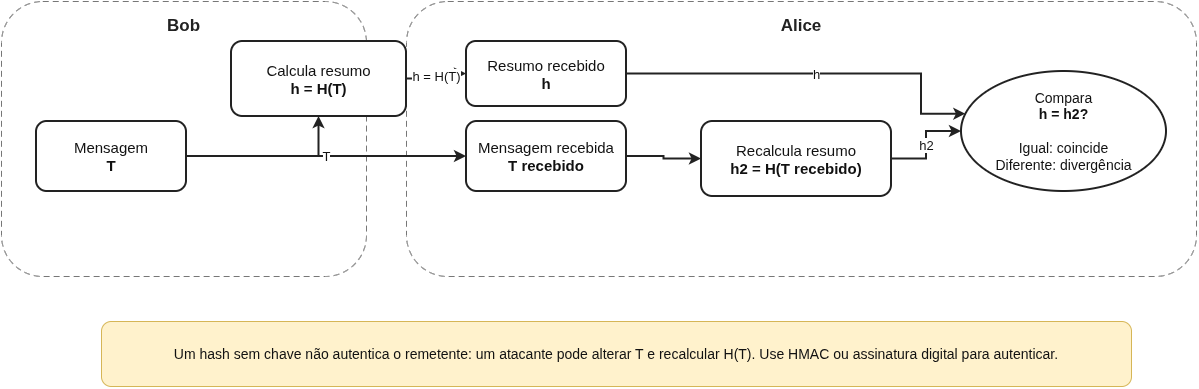
\includegraphics[scale=0.45]{hash.png}
	\caption{Funcionamento do processo de utilização do algoritmo Hash}
	\label{fig:hash}
\end{figure}

Inicialmente, \textbf{Bob} executa o algoritmo de hash sobre a mensagem e obtém o que normalmente é chamado de resumo. Tanto a mensagem quanto o resumo são enviados para \textbf{Alice}. \textbf{Alice} gera novamente o algoritmo de hash sobre a mensagem e compara o resultado do hash com o hash que foi enviado inicialmente por \textbf{Bob}. Se por acaso os valores forem iguais, então isso indica que não houve nenhum tipo de alteração na mensagem.\\

\textbf{Prático}\\

Abaixo estão exemplos de comandos utilizando o OpenSSL para realizar o processo de hash, e como é utilizado para gerar uma representação fixa de dados, independente do tamanho e do conteúdo original.

\begin{enumerate}
	\item Gerar um hash (hash.sha256) utilizando SHA-256
	\begin{tcolorbox}[width=\textwidth]
	{\small
		\begin{verbatim}
		$ openssl dgst -sha256 -out hash.sha256 arquivo.txt
		\end{verbatim}
	}
	\end{tcolorbox}

	\item Verificar a integridade de um arquivo (arquivo.txt) comparando hashes
	\begin{tcolorbox}[width=\textwidth]
	{\small
		\begin{verbatim}
		$ openssl dgst -sha256 arquivo.txt
		\end{verbatim}
	}
	\end{tcolorbox}

	\item Gerar um hash (hash.sha512) utilizando SHA-512
	\begin{tcolorbox}[width=\textwidth]
	{\small
		\begin{verbatim}
		$ openssl dgst -sha512 -out hash.sha512 arquivo.txt
		\end{verbatim}
	}
	\end{tcolorbox}

	\item Verificar a integridade de um arquivo (arquivo.txt) comparando hashes
	\begin{tcolorbox}[width=\textwidth]
	{\small
		\begin{verbatim}
		$ openssl dgst -sha512 arquivo.txt
		\end{verbatim}
	}
	\end{tcolorbox}
\end{enumerate}

\pagebreak

% Página
\section{Autenticidade}

A Autenticidade está relacionada à verificação da identidade das partes envolvidas na comunicação e à garantia de que a origem das informações é confiável. Este pilar garante que as entidades (pessoas, sistemas ou dispositivos) sejam quem dizem ser e que as informações provenientes dessas entidades sejam genuínas. Métodos de autenticação, como senhas, certificados digitais e autenticação de dois fatores, são utilizados para validar a identidade e estabelecer a confiança entre as partes. A autenticidade é crucial para prevenir fraudes e assegurar a legitimidade das transações eletrônicas.

\subsection{Assinatura Digital}

A assinatura digital é um mecanismo de segurança criptográfica fundamental para garantir a integridade e a autenticidade das informações transmitidas digitalmente.\\

\textbf{Conceito de Assinatura Digital}\\

A assinatura digital utiliza algoritmos de \textbf{criptografia assimétrica} para garantir que uma mensagem ou documento não tenha sido alterado desde que foi assinado e que realmente foi enviado pelo remetente.\\

\textbf{Funcionamento}\\

A Figura \ref{fig:assinatura} exemplifica o algoritmo de assinatura digital. Neste exemplo, Bob deseja enviar uma menagem para Alice e Bob deseja garantir que Alice possa verificar a autenticidade da mensagem.

\begin{figure}[H]
	\centering
	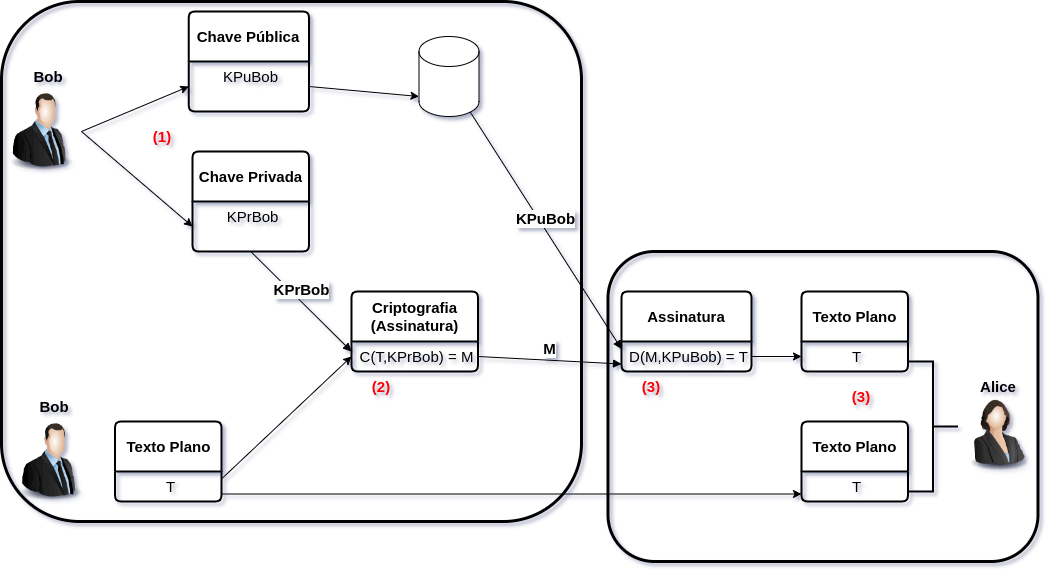
\includegraphics[scale=0.45]{assinatura.png}
	\caption{Funcionamento do processo de Assinatura Digital}
	\label{fig:assinatura}
\end{figure}

\begin{enumerate}
	\item \textbf{Criação de Chaves:}
	Bob, que deseja enviar uma mensagem assinada para Alice, primeiro cria um par de chaves criptográficas: uma chave pública(KPuBob) e uma chave privada(KPrBob);
	\begin{tcolorbox}[width=\textwidth]
		{\small
			\begin{verbatim}
			$ openssl genpkey -algorithm RSA -out KPrBob.pem -pkeyopt rsa_keygen_bits:2048
			$ openssl rsa -pubout -in KPrBob.pem -out KPuBob.pem
			\end{verbatim}
		}
	\end{tcolorbox}
	\item \textbf{Assinatura da Mensagem:}
	Bob escreve sua mensagem e, em seguida, utiliza sua chave privada para gerar uma assinatura digital. Este processo envolve a aplicação de uma função de hash na mensagem para gerar um resumo da mesma (digest). Em seguida, Bob criptografa este resumo utilizando sua chave privada. O resultado é a assinatura digital, que é enviada juntamente com a mensagem original para Alice.
	\begin{tcolorbox}[width=\textwidth]
		{\small
			\begin{verbatim}
			$ openssl dgst -sha256 -sign KPrBob.pem -out signature.bin arquivo.txt
			\end{verbatim}
		}
	\end{tcolorbox}
	\item \textbf{Verificação da Assinatura:}
	Ao receber a mensagem e a assinatura digital, Alice utiliza a chave pública de Bob para verificar a assinatura. Primeiro, ela aplica a mesma função de hash na mensagem recebida para gerar um resumo. Depois, ela utiliza a chave pública de Bob para descriptografar a assinatura digital recebida, obtendo o resumo original da mensagem assinado por Bob.
		\begin{itemize}
			\item Se o resumo gerado por Alice e o resumo obtido através da descriptografia da assinatura coincidirem, Alice pode ter certeza de que a mensagem não foi alterada e foi realmente assinada por Bob.
			\item Se os resumos não coincidirem, isso indica que a mensagem foi alterada no caminho ou que a assinatura não foi gerada pela chave privada de Bob.
		\end{itemize}
	\begin{tcolorbox}[width=\textwidth]
		{\small
			\begin{verbatim}
			$ openssl dgst -sha256 -verify KPuBob.pem -signature signature.bin arquivo.txt
			Verified OK
			\end{verbatim}
		}
	\end{tcolorbox}
\end{enumerate}

\textbf{Importância da Assinatura Digital}\\

A assinatura digital proporciona dois aspectos cruciais de segurança:

\begin{itemize}
	\item \textbf{Autenticidade:} Garante que a mensagem foi enviada pelo remetente legítimo (no caso, Bob).
	\item \textbf{Integridade:} Assegura que a mensagem não foi alterada durante a transmissão.
\end{itemize}

Em conjunto, esses aspectos permitem a confiança em comunicações eletrônicas, especialmente em transações financeiras, documentos legais e comunicação corporativa.\\

\textbf{Conclusão}\\

A assinatura digital é um componente vital na segurança da informação, oferecendo uma maneira robusta de verificar a integridade e a autenticidade de dados digitais. No exemplo de Bob e Alice, vimos como a criptografia assimétrica é utilizada para gerar e verificar assinaturas digitais, garantindo a segurança nas comunicações digitais.

\pagebreak

% Página
\section{Confidencialidade com Criptografia Híbrida}

Este exemplo demonstra confidencialidade por criptografia híbrida: Bob cifra o texto com uma chave de dados aleatória e cifra essa chave de dados com a chave pública de Alice. O fluxo não autentica Bob; para isso, seria necessário incluir uma assinatura digital ou um MAC.

\begin{figure}[H]
	\centering
	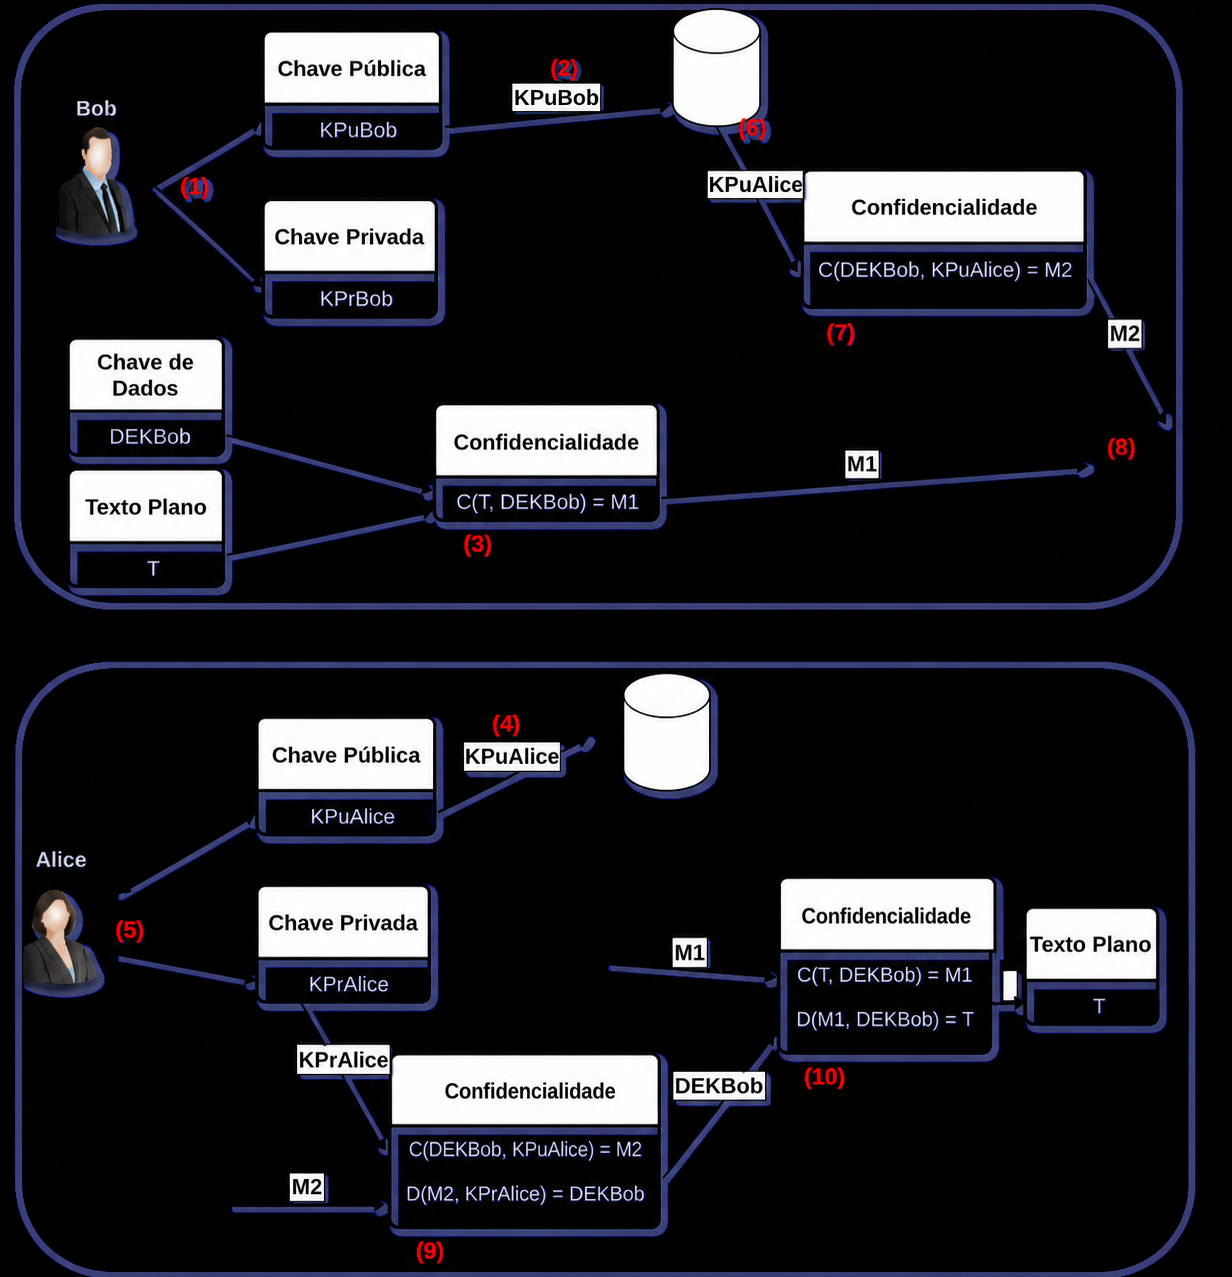
\includegraphics[scale=0.45]{confidencialidade.png}
	\caption{Confidencialidade de uma mensagem com criptografia híbrida}
	\label{fig:confidencialidade_hibrida}
\end{figure}

- \textbf{Criação das Chaves de Criptografia}

\begin{enumerate}
	\item Bob cria o seu par de chaves, Chave Pública(KPuBob.pem) e Chave Privada(KPrBob.pem);
	\begin{tcolorbox}[width=\textwidth]
		{\small
			\begin{verbatim}
			$ openssl genpkey -algorithm RSA -out KPrBob.pem -pkeyopt rsa_keygen_bits:2048
			$ openssl rsa -pubout -in KPrBob.pem -out KPuBob.pem
			\end{verbatim}
		}
	\end{tcolorbox}
	\item Bob envia a sua Chave Pública(KPuBob.pem) para o servidor;
	\item Alice cria o seu par de chaves, Chave Pública(KPuAlice.pem) e Chave Privada(KPrAlice.pem);
	\begin{tcolorbox}[width=\textwidth]
		{\small
			\begin{verbatim}
			$ openssl genpkey -algorithm RSA -out KPrAlice.pem -pkeyopt rsa_keygen_bits:2048
			$ openssl rsa -pubout -in KPrAlice.pem -out KPuAlice.pem
			\end{verbatim}
		}
	\end{tcolorbox}
	\item Alice envia a sua Chave Pública(KPuAlice.pem) para o servidor;
\end{enumerate}

- \textbf{Cifragem híbrida (Bob)}

\begin{enumerate}
	\setcounter{enumi}{4} % Define o contador para começar do número 5
	\item Bob gera uma Chave de Dados (DEKBob.bin) e a utiliza para cifrar o Texto Plano, gerando o Texto Cifrado M1;
	\begin{tcolorbox}[width=\textwidth]
		{\small
			\begin{verbatim}
				# Gerar uma chave simétrica (DEKBob.bin)
				$ openssl rand -out DEKBob.bin 32
				
				# Criptografar T.txt usando a chave bruta DEKBob.bin e um IV aleatório
				$ DEK_HEX=$(od -An -v -tx1 DEKBob.bin | tr -d ' \n')
				$ IV_HEX=$(openssl rand -hex 16)
				$ printf '%s' "$IV_HEX" > M1.iv
				$ openssl enc -aes-256-cbc -K "$DEK_HEX" -iv "$IV_HEX" \
				  -in T.txt -out M1.enc
			\end{verbatim}
		}
	\end{tcolorbox}
	\item Bob recupera a Chave Pública da Alice(KPuAlice)
	\item Bob cifra a sua Chave de Dados (DEKBob.bin) com a Chave Pública da Alice (KPuAlice.pem), gerando o Texto Cifrado M2;
	\begin{tcolorbox}[width=\textwidth]
		{\small
			\begin{verbatim}
				# Criptografar a chave AES usando a chave pública de Alice (KPuAlice.pem)
				$ openssl pkeyutl -encrypt -in DEKBob.bin -inkey KPuAlice.pem -pubin -out M2.enc \
				  -pkeyopt rsa_padding_mode:oaep -pkeyopt rsa_oaep_md:sha256
			\end{verbatim}
		}
	\end{tcolorbox}
	\item Bob envia o Texto Cifrado M1 e M2 para o servidor;
\end{enumerate}

- \textbf{Decifragem (Alice)}

\begin{enumerate}
	\setcounter{enumi}{8} % Define o contador para começar do número 10
	\item Alice descriptografa o Texto Cifrado M2 com sua Chave Privada (KPrAlice.pem) para obter a Chave de Dados (DEKBob.bin);
	\begin{tcolorbox}[width=\textwidth]
		{\small
			\begin{verbatim}
			$ openssl pkeyutl -decrypt -in M2.enc -inkey KPrAlice.pem -out DEKBob.bin \
			  -pkeyopt rsa_padding_mode:oaep -pkeyopt rsa_oaep_md:sha256
			\end{verbatim}
		}
	\end{tcolorbox}
	\item Alice descriptografa o Texto Cifrado M1 com a DEK do Bob (DEKBob.bin) e o IV associado para obter o Texto Plano (T);
	\begin{tcolorbox}[width=\textwidth]
		{\small
			\begin{verbatim}
			$ DEK_HEX=$(od -An -v -tx1 DEKBob.bin | tr -d ' \n')
			$ openssl enc -d -aes-256-cbc -K "$DEK_HEX" -iv "$(cat M1.iv)" \
			  -in M1.enc -out T.txt
			\end{verbatim}
		}
	\end{tcolorbox}
\end{enumerate}

\pagebreak

%Copyright
\vspace*{\fill}
\begin{flushright}
	\underline{\textit{Copyright}}\\
	All rights reserved to MT4 Tecnologia LTDA.\bigskip

	\underline{\textit{Propósito deste documento}}\\
	Conceitos de criptografia\bigskip

	\underline{\textit{Versão}}\\
	Versão 1.0\bigskip

	\underline{\textit{Autor}}\\
	Caio Abreu Ferreira [\href{mailto:cferreira@senhasegura.com}{cferreiras@senhasegura.com}] \bigskip\\
	
	\underline{\textit{MT4 Tecnologia Ltda.}}\\
	Rua Joaquim Antunes, 767 – Pinheiros – São Paulo\\
	Phone: +55 11 3065-7070\\
	\url{www.mt4.com.br}\\
	\href{mailto:support@senhasegura.com}{support@senhasegura.com}\\
\end{flushright}

\end{document}
